\section{Research}

\subsection{System architecture}

\subsubsection{System overview}

\begin{figure}
  \centering
  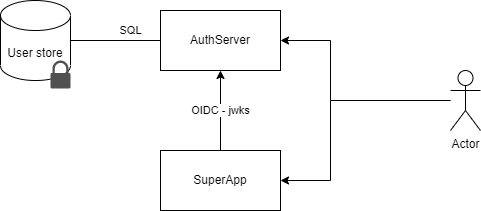
\includegraphics[scale=0.65]{architecture/initial.png}
  \caption{Initial system architecture}
  \label{fig:sys-highlevel}
\end{figure}


\paragraph{Initial state}

In figure \ref{fig:sys-highlevel} we see a high-level overview of a system we are trying to integrate eID authentication. This system consists of the following components:

\begin{enumerate}
  \item AuthServer - the company's SSO; acts as a central authority for identity. Issued OIDC id tokens, which contain user ID, their roles, and claims.
  \item SuperApp - a resource server with access control enabled. It uses id tokens issued by AuthServer and verifies them using asymmetric cryptography.
  \item User store - a data store containing user login information - usernames, password hashes, other PII.
  \item Actor - a physical person accessing the resources in the system.
\end{enumerate}

\paragraph{Desired state}

The company wishes to implement eID authentication. Since the authentication is not done locally but is delegated to some remote service or device, the protocol can be treated as an external federated sign-in. Frameworks such as ASP.NET Identity have special helpful tools to handle external identity providers.

With the inclusion of an external eID provider, we can see the new system architecture in figure \ref{fig:sys-highlevel-witheid}.

\begin{figure}
  \centering
  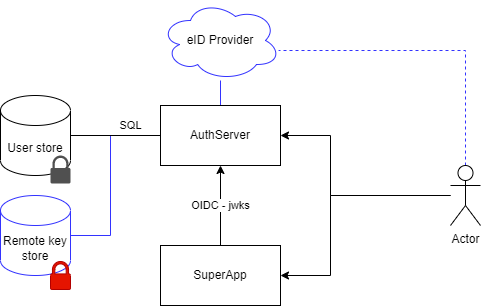
\includegraphics[scale=0.65]{architecture/witheid.png}
  \caption{System architecture after the inclusion of an eID provider}
  \label{fig:sys-highlevel-witheid}
\end{figure}

We can see two significant additions:

\begin{enumerate}
  \item eID provider - a gateway to obtain someone's eID. It can be any eID source like Dokobit, TARA, Smart-ID, ID card.
  \item Remote key store - it is a storage for unique identifiers provided by the eID provider.
\end{enumerate}

The primary purpose of the remote key store is to link the user ID used in the internal system with the unique identifier provided by the eID provider. Because the unique identifier can change or the same physical person can have multiple eIDs \cite{eidas-saml}, it is required to allow numerous eIDs to map to a single internal ID.

The key store is represented with the addition of a red lock. Depending on the country, the data stored there may be subject to strict privacy regulations. Companies should consider implementing strict access control for this part of the infrastructure.

\paragraph{Final state}

The end goal for the scope of this thesis is to implement three eID providers into the architecture. For normal companies, it would make sense to implement multiple in case they would like to get more coverage. Additionally, they could register non eID providers, such as Google or Microsoft social logins. The final high-level overview of the system can be seen in figure \ref{fig:sys-highlevel-final}.

\begin{figure}
  \centering
  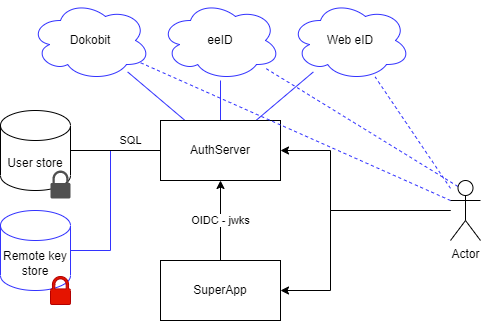
\includegraphics[scale=0.65]{architecture/final.png}
  \caption{System architecture after the inclusion of all eID providers in scope}
  \label{fig:sys-highlevel-final}
\end{figure}

\subsubsection{Process overview}

For validation of the architecture, we will consider two use cases.

The first one (see figure \ref{fig:sysprocess-a}) is concerned about accessing a protected resource with a token issued by the AuthServer. This use case validates the base state of the system.

The second use case (see figure \ref{fig:sysprocess-b}) is also concerned about accessing a protected resource, but only those, who authenticate with a higher level of assurance, like eID, can access it. This use case validates the successful implementation of eID authentication and access control.

\begin{figure}
  \centering
  \begin{sequencediagram}
    \newthread{A}{Actor}{}
    \newinst[3]{B}{AuthServer}{}
    \newinst[1]{C}{SuperApp}{}

    \begin{call}{A}{accessProtected()}{C}{401 Unauthorized}\end{call}

    \begin{call}{A}{authWithPassword()}{B}{Auth token}\end{call}
    \begin{call}{A}{accessProtected()}{C}{Data}\end{call}
    \begin{call}{A}{accessReallyProtected()}{C}{403 Forbidden}\end{call}
  \end{sequencediagram}
  \caption{System behavior when authenticated with a username + password scheme}
  \label{fig:sysprocess-a}
\end{figure}

\begin{figure}
  \centering
  \begin{sequencediagram}
    \newthread{A}{Actor}{}
    \newinst[2]{B}{AuthServer}{}
    \newinst[1]{C}{SuperApp}{}

    \begin{call}{A}{accessProtected()}{C}{401 Unauthorized}\end{call}

    \begin{call}{A}{authWithEid()}{B}{Auth token}\end{call}
    \begin{call}{A}{accessProtected()}{C}{Data}\end{call}
    \begin{call}{A}{accessReallyProtected()}{C}{Very Secret Data}\end{call}
  \end{sequencediagram}
  \caption{System behavior when authenticated with an eID scheme}
  \label{fig:sysprocess-b}
\end{figure}

\subsubsection{Linking eID to an internal user ID}

There will be a need to uniquely link an identity to an internal account in the company SSO. The security requirement, in this case, is not to allow other users to access the same account. For this goal, companies must use one or more person-identifying properties.

When using a passport as a reference, it has the following identifiers: (issuer) country code, document number, surname, given name, personal code, citizenship, date of birth, date of issue, date of expiry, and authority. In these cases, it is easy to use the personal code for identifying a person as it is unlikely to change - people change names, documents expire; authorities and date of birth do not narrow it down nearly enough.

Implementers will hit a roadblock when checking a passport of Ireland - additionally, it has a place of birth but, more importantly, no personal identification code. In this case, the next best unique identifier would be to use the document number and update the account with a new number when the document eventually expires and is replaced.

In the world of digital identity, the eIDAS node network must provide a unique identifier for all requests \cite{eidas-saml}. Having a standardized way of obtaining an identifier is good news. All countries who wish to connect to the eIDAS network would have to expose some code to identify a person uniquely, removing the burden from the software architects to analyze what identifier they should use.

In the eIDAS node network, the unique identifier remains "unchanged for the lifetime of the account" \cite{eidas-saml}. Unfortunately, it does not mean that identifiers cannot change; the account associated with that identifier cannot change. If an identifier were to change when "the user's digital identity is replaced or repaired," relying parties should treat the newly obtained identifier as a completely new identity.

\paragraph{eIDAS Unique Identifier Structure} In eIDAS SAML Attribute Profile, an identifier code is defined as:
\begin{enumerate}
  \item The first part is the Nationality Code of the identifier. This is one of the ISO 3166-1 alpha-2 codes, followed by a slash ("/")).
  \item The second part is the Nationality Code of the destination country or international organization. This is one of the ISO 3166-1 alpha-2 codes, followed by a slash ("/").
  \item The third part is a combination of readable characters. This uniquely identifies the identity asserted in the country of origin but does not necessarily reveal any discernible correspondence with the subject's actual identifier (for example, username, fiscal number etc).
\end{enumerate}

Example: ES/AT/02635542Y (Spanish eIDNumber for an Austrian SP).

\paragraph{Summary} Using eIDAS Unique Identifier structure as a base, we can see that it is enough to uniquely identify a digital identity in eIDAS with the country of origin, country of destination, and a set of characters to identify that person in the origin country. The destination country will always be the same in our company's case. To uniquely identify a person, we will only need its origin country and a unique identifier a member state must provide.

For this thesis, identifiers will be marked as "{\{ISO 3166-1 alpha-2\}}/{\{Code provided by country\}}". Unique identifier examples: EE/38001085718, LT/49003111045, SE/870314-2391.

\subsubsection{Privacy Policy}

The company wishing to implement eID authentication will have to deal with personal information as described by GDPR \cite{eulaw-gdpr}. Before going live with an eID solution, companies must first consult a legal professional for advice.

A privacy policy is a legal document and is way outside of the scope of a technical implementation thesis. However, it is still important to understand the basics. For this goal, two privacy policies will be analyzed: Web eID \cite{legal-webeid-privacypolicy} and Dokobit \cite{legal-dokobit-privacypolicy}.

From the cursory analysis of the two policies, there are three fundamental aspects our company needs to address: what data is processed, with whom the company shares the data, and what is the retention policy.

Based on the privacy policies of Web eID and Dokobit, we constructed a rudimentary privacy policy for the use of the test application environment. A copy of the text can be found in the thesis' appendices.

Further research can be done to outline better the GDPR requirements needed to process a person's eID.

\subsection{Weaknesses in the architecture}

All systems come with points of compromise. It is best to be aware of these weak points and harden against them early on rather than after a cyber incident. The weaknesses can be grouped into two parts: eID provider dependent and local.

\paragraph{eID provider dependant weaknesses}

These threats come from one common issue: trusting an eID service provider when a relying party should not have. There are four primary causes:

\begin{enumerate}
  \item relying party trusts an input from an insecure channel;
  \item relying party does not perform the necessary validation;
  \item weakness in the architecture of transport protocol;
  \item eID provider itself gets compromised;
\end{enumerate}

These points will be addressed on a case-by-case basis for each of the eID providers in the study.

\paragraph{Local weaknesses}

In figure \ref{fig:sys-highlevel-witheid}, four components are not linked to a particular eID: AuthServer, SuperApp, application store, user store, and remote key store. We can identify weaknesses for those parts here. Each weakness was analyzed through the lens of CIA security analysis.


\subsubsection{SuperApp}

These two assets have similar weaknesses, with the only difference being the way users authenticate themselves. More in-depth analysis on authentication for the AuthServer can be seen on the 

\paragraph{[CI] Users can see and or edit data normally forbidden to access} This issue is usually created by one of two causes:

\begin{enumerate}
  \item access control measures are disabled or do not protect resources;
  \item OIDC token validation is disabled or misconfigured;
\end{enumerate}

The first cause has a trivial fix - developers have likely forgotten to enable the data access guard on the endpoint. It is unlikely that all authorization rules break.

In the case of the second cause, some corners were likely cut in the ID token validation process. When validating a token, the process has to match the one described in the OIDC spec \cite{oidc} exactly. This process consists of three major parts:

\begin{enumerate}
  \item check if the token's crypto algorithm is as expected;
  \item validate token signature;
  \item validate claims - issuer, audience, timestamp, nonce;
\end{enumerate}

Developers usually need not worry about the process, as most frameworks have adopted the OpenID Connect protocol or have well-maintained libraries.

\paragraph{[A] Service becomes unavailable} This threat is caused by one of the following:

\begin{enumerate}
  \item server is offline or overloaded;
  \item OIDC token validation is misconfigured to have an incorrect authority;
\end{enumerate}

The first case is a common availability issue, meaning the server is suffering a denial of service attack. We will not cover the mitigation of this form of availability threat in the scope of the thesis.

A likely cause for this issue is the manually configured OIDC properties on the relying party. If possible, developers should never configure the properties manually and use the well-known metadata endpoint instead. A metadata endpoint usually looks like this - \url{https://auth.mycompany.org/.well-known/openid-configuration}.


\subsubsection{AuthServer}

All of the points that apply to SuperApp also apply to AuthServer. However, there is a critical use case that is worth mentioning explicitly.

\paragraph{[CI] Users can see used eID schemes and add new ones with unsafe sign-in}

As per requirements, users must assign multiple identity providers to their accounts. When adding a new external scheme, the currently signed-in user must have the same privilege level as the scheme they are trying to add. This countermeasure is for the event an adversary gains access to their account; they wouldn't be able to elevate their privileges by adding their eID scheme and signing in with it.

With this requirement in place, registration with an email and password becomes less valuable, as those accounts could never add an eID afterward. An exception to this rule can occur if a user has no eID schemes registered.

This problem is solved by having a company policy to verify the user's first added eID manually. Without this verification, an adversary can register a new account with their real eID and access the data anyway.

\subsubsection{Data stores}

All three data stores have the exact issues between them. For the sake of brevity, they will be grouped under the umbrella of \textit{data store}.

\paragraph{[CI] Users have a less secure way of accessing the data store}

The system is as secure as its weakest link. If users have direct access to the database while bypassing the eID authentication check, the security and assurance guarantees are worthless.

If there are alternative ways of accessing the database, companies must implement proper access rules that would be as secure as the one's eIDs provide. How that can be achieved depends on what data storage option is being used. The best option would be to close down external access to the data stores completely.

\paragraph{[CI] Man-in-the-middle attacks} While uncommon, some data stores are vulnerable to MitM attacks \cite{sql-server-auth-mitm}. Although the best course of action would be to move the data storage server away from the general internet and make it accessible only on the local network or VPN, that is not always enough. For maximum security, companies must implement the recommended MitM prevention techniques \cite{sql-server-enable-tls}.

\paragraph{[A] Data is destroyed or lost}

Ransomware attacks and accidental database corruptions can happen, so offline remote backups are a must.

One must not forget to satisfy the requirement of not allowing for easier access to data even here. These backups must be protected from unauthorized access.

One approach to solving this would be to use encryption; keys should only be available after authenticating with an eID scheme. One equally secure alternative would be to use something like the encryption and decryption functionality of Estonia's ID cards.

\subsection{Case Study: Dokobit}

\subsubsection{About}

Dokobit \cite{dokobit}, trademark and subsidiary of Estina \cite{euipo-dokobit}, offers two products: Document Signing Portal and API solutions.

The first product, the Document Signing Portal, was released in 2014 \cite{dokobit-aboutus}. The primary purpose of this solution is to allow users to upload documents and digitally sign them online.

Estina has acquired the DigiDoc portal (\url{https://digidoc.ee}) from SK ID Solutions in 2016 \cite{sk-digidocacquired} which had the exact purpose. This portal should not be confused with the similarly named DigiDoc4 client Estonians commonly use to sign documents \cite{ria-idee}.

The second product, API solutions, targets businesses in a variety of scopes: signature collection, signing, identification, sealing, and TSP monitoring \cite{dokobit}. In the thesis, we will only consider the Identification service.

Dokobit's Identification service allows Lithuanian, Latvian, Estonian, Finnish, Norwegian, Icelandic, Polish, Belgian, Portuguese, Spanish, and Italian \cite{dokobit} users to authenticate themselves with their countries' scheme. It is the highest country count and market reach of all three case studies.

The company has received ISO/IEC 27001:2013 certification \cite{dokobit-certification} and in 2020 was included in the EU Trusted Service List \cite{eu-trustservices, dokobit-aboutus}, thus it becoming a Qualified Trust Service Provider.

In 2021, the Norwegian electronic identity solutions provider company Signicat AS acquired UAB Dokobit.

\subsubsection{Dokobit Identification Service}

Identification service supports two distinct data flows: Gateway and API. The core difference between them is that the Gateway uses a prebuilt UI on their server. In contrast, the API requires the companies to develop their UI and have their server communicate with Dokobit servers instead. This difference only affects the user experience.

The main advantage of Identity Gateway over Identity API is the added brand trust. A study finds that users "associate higher security feelings with a higher level of brand trust" \cite{ha2004factors}. If an organization has not matured yet as a brand (such as a recent startup), it will make more sense for them to choose Identity Gateway over API. On the contrary, if they are a large, highly trusted organization, such as a bank, it would make more sense to use Identity API and have all user interactions happen on the same domain.

For this thesis, we will only analyze the Identity Gateway in depth.

\paragraph{Embed or Redirect}

Identity Gateway comes in two primary user flows: embedded and redirect-based.

In embedded flow, users could stay on the website, authenticate in a pop-up modal, and update the website view accordingly after finishing the authentication process. Embedded flow has the advantage of not requiring the users to leave the website, which is helpful to preserve user data in complex forms.

In redirect-based flow, users are sent to an external website, perform authentication, and redirect to the company website, in a flow similar to OAuth2.

Ultimately, experts consider the embedded flow to be the weaker of the two methods \cite{auth0-universal-vs-embedded} for two main reasons:

\begin{enumerate}
  \item Cross-origin requests are inherently more dangerous, allowing for MitM and CSRF attacks;
  \item The client application, even when embedded, receives full client credentials, which adds another point of compromise in the form of XSS;
\end{enumerate}

When using federated sign-in for Native Apps, "best current practice requires that native apps MUST NOT use embedded user-agents to perform authorization requests" \cite{rfc8252}. This practice means that companies who have a mobile app or would consider having one in the future mustn't use Embedded flow.

\subsubsection{Data Flow}

This section will analyze Dokobit Identity Gateway, redirect-based user flow, the general overview of which can be seen in figure \ref{fig:dokobit-identitygw-redirect}. We can group the authentication process into three parts: establishing a session with Dokobit, user authentication with an eID provider, and user information retrieval.

\begin{figure}
  \centering
  \begin{sequencediagram}
    \newthread{A}{Actor}{}
    \newinst[2]{B}{AuthServer}{}
    
    \newinst[1]{C}{IDGW Backend}{}
    \newinst[1]{D}{IDGW Frontend}{}

    \begin{call}{A}{1. authenticate()}{B}{Session}
      \begin{call}{B}{2. POST /api/authentication/create}{C}{session\_token}\end{call}
      \begin{call}{B}{3. HTTP 302 Redirect}{D}{HTTP 302 Redirect}
        \begin{call}{D}{4. renderedAuthForm()}{A}{Credentials}\end{call}
      \end{call}

      \begin{call}{B}{5. GET /api/authentication/\{session\_token\}/status}{C}{User data}\end{call}
    \end{call}
  \end{sequencediagram}
  \caption{Dokobit Identity Gateway - Redirect-based user flow \cite{dokobit-idgw-docs}}
  \label{fig:dokobit-identitygw-redirect}
\end{figure}

\paragraph{Establishing a session with Dokobit}

When a user requests to authenticate, the company's back-end systems' first step is to establish a session with Dokobit Identity Gateway. To do this, a {POST} request must be made to the {/api/authenticate/create} endpoint. This response will contain the session identifier and the redirect URL. Users will have to go there to interface with their eID providers.

\paragraph{User authentication with an eID provider}

After the back-end successfully creates a session, they must redirect the user to the received endpoint. An easy way to accomplish that is to respond to the initial authentication request with HTTP status 302 - Found.

Most of the heavy lifting with authentication is delegated to this step and handled by Dokobit. The company's back-end systems should wait for the user to return after authenticating.

\paragraph{User information retrieval}

After the user returns after successful authentication, the back-end servers should make a {GET} request to {/api/authentication/session\_token/status} endpoint. From there, the company can securely receive the user information via a backchannel.

\subsubsection{Trust Anchor}


\subsubsection{Pricing}
\subsubsection{Security Analysis}

\subsection{Case Study: eeID}

\subsubsection{About}
\subsubsection{Data Flow}
\subsubsection{Trust Anchor}
\subsubsection{Pricing}
\subsubsection{Security Analysis}

\subsection{Case Study: Web eID}

\subsubsection{About}

Released in the Summer of 2021 \cite{ria-webeid} and having undergone significant changes in January of 2022, this eID framework allows users to authenticate and sign documents using their smart cards.

Functionally this framework is split into three parts: software the user needs to install on their computer, a javascript library that acts as a data intermediary, and the certificate validation library for the back-end.

The software users need to install is similar to the one various countries' governments issue. The significant difference is that this software supports more than one countries' eID solutions. Supported countries include Estonia, Latvia, Lithuania, and Finland \cite{ria-webeid}.

This service is built by the Estonian Information System Authority, responsible for TARA, Estonia's public sector gateway. No publicly available audit certification is available at the time of writing \todo{is this true?}.

\subsubsection{Data Flow}

Figure \ref{fig:web-eid-authentication} displays the high-level overview of the complete flow of data within the Web eID framework. A detailed explanation of the steps can be found on the technical specification page \cite{ria-webeid-systemarchitecture}. Companies implementing the framework should only consider the browser and the server application (steps 1-3 and 13-17).

\begin{figure}
  \centering
  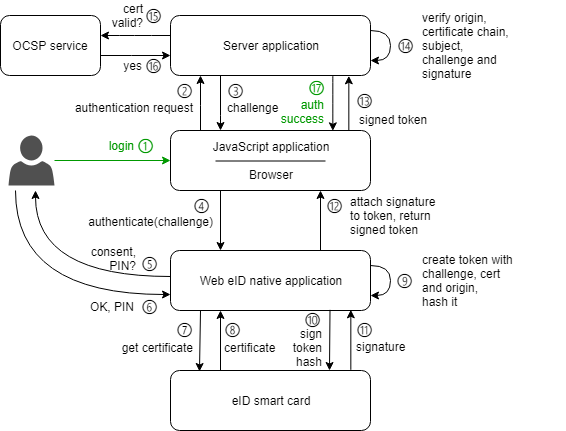
\includegraphics[scale=0.6]{webeid/Web-eID-authentication-communication-diagram}
  \caption{Web eID Authentication flow \cite{ria-webeid-systemarchitecture}}
  \label{fig:web-eid-authentication}
\end{figure}

\subsubsection{Trust Anchor}

Unlike Dokobit and eeID, Web eID does not provide any guarantees about the trustworthiness of a certificate. It is, however, not out of malice and reminds developers by sending the certificate in a field called "unverifiedCertificate" \cite{ria-webeid-source-web-eid-authtoken-validation-java-readme}.

The relying party must verify the certificate and challenge themselves by checking the origin, certificate expiry, trust chain, OCSP response, and the challenge. This validation structure makes the trust anchor technological and highly dependent on the implementation correctness by the developers.

\todo{Discuss how we can never trust developers without proper supervision}

\subsubsection{Pricing}

The Web eID authentication service is free of charge, as the only external validation, OCSP \cite{rfc6960} requests are free to use. When creating digital signatures, the timestamping service may require payment \cite{ria-webeid-source-web-eid-authtoken-validation-java-readme}.

\subsubsection{Security Analysis}

\paragraph{Actors}

The actors in the figure \ref{fig:eid-auth-flow-seq} assume the roles of: QSCD Interface - web-eid.js \cite{ria-webeid-source-web-eid-js}, web-eid-app \cite{ria-webeid-source-web-eid-app}; QSCD - Smart cards of Estonia, Latvia, Lithuania, and Finland \cite{ria-webeid}.

Even though distributed by the same website, id.ee, this interface is separate from the official id.ee software Estonian citizens use to sign and verify documents. "In the future, the final version of Web eID will be added into the ID-software installation package, available for the users the website on www.id.ee" \cite{ria-webeid}. Owners of other countries' smart cards will still have to download the special software from id.ee.

\paragraph{Communication channel}

The Web eID framework uses an insecure channel for communications, so developers must take caution and verify received data when implementing the framework. This channel is susceptible to man-in-the-middle attacks done by the client.

Unlike in the cases of Dokobit and eeID, the risk of impersonation is not transferred to the eID service provider.

\paragraph{Validation requiements}

For each protocol implementation step, developers will have to fulfill certain guarantees before the system goes into production.

\subparagraph{Steps 1-3}

Building the challenge nonce. The goal of these steps is to create the challenge the user will have to sign with their private key. There are a couple of guarantees the application must provide:
\begin{enumerate}
  \item Generated challenge nonce must be between 32 and 96 bytes (inclusive) in length \cite{ria-webeid-source-web-eid-app-authenticate};
  \item "It must be guaranteed that the authentication token is received from the same browser to which the corresponding challenge nonce was issued" \cite{ria-webeid-source-web-eid-authtoken-validation-java-readme}. The framework creators suggest attaching it to the user session.
  \item "Cache must be used for protection against replay attacks by guaranteeing that each authentication token can be used exactly once" \cite{ria-webeid-source-web-eid-authtoken-validation-java-readme}.
  \item "Cookie-based authentication must be protected against cross-site request forgery (CSRF) attacks and extra measures must be taken to secure the cookies by serving them only over HTTPS and setting the HttpOnly, Secure and SameSite attributes" \cite{ria-webeid-source-web-eid-authtoken-validation-java-readme}.
\end{enumerate}

In the implementation example, these measures were addressed by:
\begin{enumerate}
  \item a 64 byte cryptographically secure randomly generated nonce is created (see listing \ref{lst:web-eid-challenge});
  \item challenge nonce is set in the user's session, which adversaries cannot tamper;
  \item the generated nonce is stored into local memory cache for later use; nonce expires after 5 minutes;
  \item an input field is rendered on the page with a unique CSRF validation token, which prevents cross-site request forgery attacks (see listing \ref{lst:web-eid-challenge-ui});
\end{enumerate}

\begin{lstlisting}[caption={Web eID Challenge Endpoint}, label={lst:web-eid-challenge}]
private TimeSpan ChallengeLifetime { get; } = TimeSpan.FromMinutes(5);

private readonly IMemoryCache _cache; // Injected

[HttpGet("challenge")]
public IActionResult GetChallenge()
{
    var nonce = RandomNumberGenerator.GetBytes(64);

    _cache.Set(Convert.ToBase64String(nonce), true, ChallengeLifetime);
    HttpContext.Session.Set("eid.challenge", nonce);

    return Ok(new { nonce });
}
\end{lstlisting}


\begin{lstlisting}[caption={Web eID UI excerpt}, label={lst:web-eid-challenge-ui}, language={html}]
@inject Microsoft.AspNetCore.Antiforgery.IAntiforgery _csrf
@{ var csrfToken = _csrf.GetAndStoreTokens(HttpContext); }

<!-- Button used to sign in -->
<a role="button" class="btn btn-secondary" id="webeid-auth-button">Web eID</a>

<input id="csrfToken" type="hidden" value="@csrfToken.RequestToken"/>

<script>
    ...

    const authTokenResponse = await fetch("/signin-id/login", {
        method: "POST",
        headers: {
            "Content-Type": "application/json",
            "RequestVerificationToken": document.getElementById("csrfToken").value
        },
        body: JSON.stringify(...)
    });

    ...
</script>
\end{lstlisting}

\subparagraph{Steps 13-17}

After the user signs the nonce challenge and sends their certificate, the server must verify its authenticity. The application must perform all of the following before allowing the user to sign in:

\begin{enumerate}
  \item verify the CSRF token from earlier steps \cite{ria-webeid-source-web-eid-authtoken-validation-java-readme};
  \item verify the challenge nonce came from the original user and has not expired, was not consumed;
  \item verify the certificate validity and check if nonce was signed by the associated private key (see below);
  \item issue an authentication token with the fields from the certificate's subject;
\end{enumerate}

In the implementation example, these measures were addressed by:
\begin{enumerate}
  \item the back end endpoint for login is decorated with ValidateAntiForgeryToken Attribute. This attribute instructs the ASP.NET API to ignore requests not containing a CSRF token \cite{msdocs-anti-request-forgery}. A JavaScript application can only access the protected endpoints by providing RequestVerificationToken header (see listing \ref{lst:web-eid-challenge-ui});
  \item the application tries to extract the challenge nonce from the browsing session. The process would succeed if the session cookie were not modified. After the extraction, the application checks the nonce cache to verify if the challenge is still active. Cache hit means the nonce has not expired, and no previous authentication attempt was performed. Remove the challenge nonce from all stores.
  \item The API calls a standalone validation service to verify the nonce and certificate (see below).
  \item Application populates the ASP.NET identity management system with the fields from the certificate: serial number, given name, surname, country. An identity session cookie is sent to the client.
\end{enumerate}

\begin{lstlisting}[caption={Web eID Login Endpoint}, label={lst:web-eid-login}]
[HttpPost("login")]
[ValidateAntiForgeryToken]
public async Task<IActionResult> Login([FromBody] WebIdAuthTokenResponse token)
{
    // Obtain the challenge from session
    if (!HttpContext.Session.TryGetValue(ChallengeNonceKey, out var nonce) && nonce == null)
        return Unauthorized();

    // Check if token was not used before or expired
    var challenge = Convert.ToBase64String(nonce);
    if (!_cache.TryGetValue(challenge, out _))
        return Unauthorized();

    _cache.Remove(challenge);
    HttpContext.Session.Remove(ChallengeNonceKey);

    // Validate the certificate and signed challenge
    var validationResult = await _webEidValidationService.GetResult(new WebEidValidationRequest(token, nonce));
    if (!validationResult.Success)
        return Forbid();

    // Certificate is valid. Sign in the user

    await HttpContext.SignInAsync(BuildUser(new X509Certificate2(Convert.FromBase64String(token.UnverifiedCertificate)).Subject));

    return Ok();
}
\end{lstlisting}

\subparagraph{Certificate and nonce verification}

This step is the most complicated in the entire validation process. To prevent any issues with incorrect implementation, the framework maintainers recommend using their library for validation \cite{ria-webeid-source-web-eid-authtoken-validation-java-readme}. Libraries can come with security vulnerabilities, and developers are reluctant to update their used version; however, it is still more favorable to creating vulnerabilities from misconfiguration \cite{9240619}.

The eu.webeid.security Java package performs most of the certificate validation: expiry, purpose, policy, OCSP \cite{ria-webeid-source-web-eid-authtoken-validation-java-readme}. Developers will only have to configure the CA and host validation. Configuration is handled by providing a set of trusted CA certificates for trust chain verification and the hostname for challenge nonces (see listing \ref{lst:web-eid-java-lib}).

\todo{This library does favor EE cards a lot more, even having hardcoded some Mobile ID policies. Not sure if it is worth mentioning.}

\begin{lstlisting}[caption={Web eID Login Endpoint}, label={lst:web-eid-java-lib}]
public class AuthTokenValidatorService {

  @Bean
  public AuthTokenValidator validator() {
    try {
      return new AuthTokenValidatorBuilder()
        .withSiteOrigin(URI.create(System.getenv("ORIGIN_URL")))
        .withTrustedCertificateAuthorities(loadTrustedCACertificatesFromCerFiles())
        .build();
    } catch (JceException e) {
      throw new RuntimeException("Error building the Web eID auth token validator.", e);
    }
  }

  private X509Certificate[] loadTrustedCACertificatesFromCerFiles() {
    List<X509Certificate> caCertificates = new ArrayList<>();

    try {
      CertificateFactory certFactory = CertificateFactory.getInstance("X.509");

      File[] files = new File("/certs").listFiles((f, n) -> n.endsWith(".cer"));
      if (files != null) {
        for (File file : files) {
          try (InputStream stream = new FileInputStream(file)) {
            X509Certificate caCertificate = (X509Certificate) certFactory.generateCertificate(stream);
            caCertificates.add(caCertificate);
          }
        }
      }
    } catch (CertificateException | IOException e) {
      throw new RuntimeException("Error initializing trusted CA certificates.", e);
    }

    return caCertificates.toArray(new X509Certificate[0]);
  }
}
\end{lstlisting}

The token validation service described in listing \ref{lst:web-eid-java-lib} requires the maintainers to set the origin URL in the form of an environment variable and to populate the folder {/certs} with trusted CA certificates.

Origin URL can be obtained by checking the {window.origin} JavaScript variable in the page containing the sign-in button.

For the CA certificate set, the company can get an up-to-date list of trusted certificates at the EU Trust Services Dashboard \cite{eu-trustservices}. The issue with this list is that it contains all trust certificates for various scopes. In our case, we should limit the search to the extent of QCert for ESig. In the case of Estonia and Lithuania, only three entities are certified to issue certificates for QSCD (see figure \ref{fig:eu-tsp-list}). It is in stark contrast to Spain's 31 \cite{eu-trustservices}. It is possible to further narrow down to only certificate generation services for qualified certificates (CA/QC).

\begin{figure}
  \centering
  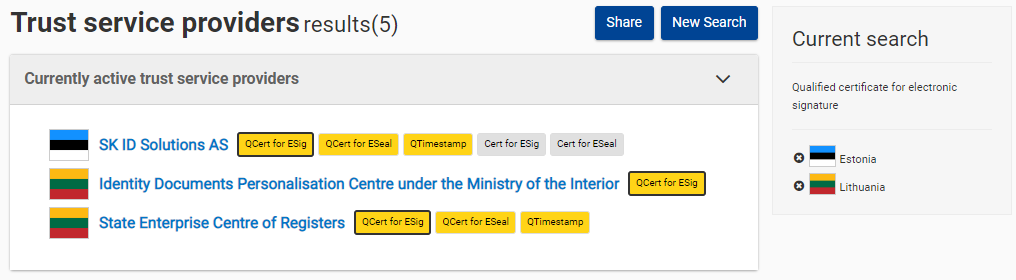
\includegraphics[scale=0.54]{webeid/eu-tsp-search}
  \caption{List of EU Trust service providers of Estonia and Lithuania capable of creating qualified certificates for e-signatures}
  \label{fig:eu-tsp-list}
\end{figure}

In the case of Estonia's single TSP, we can see that only 3 CA are currently operational (see figure \ref{fig:eu-tsp-skid}). Unfortunately, there is no standardized way of narrowing down which certificates could be used for authentication.

\begin{figure}
  \centering
  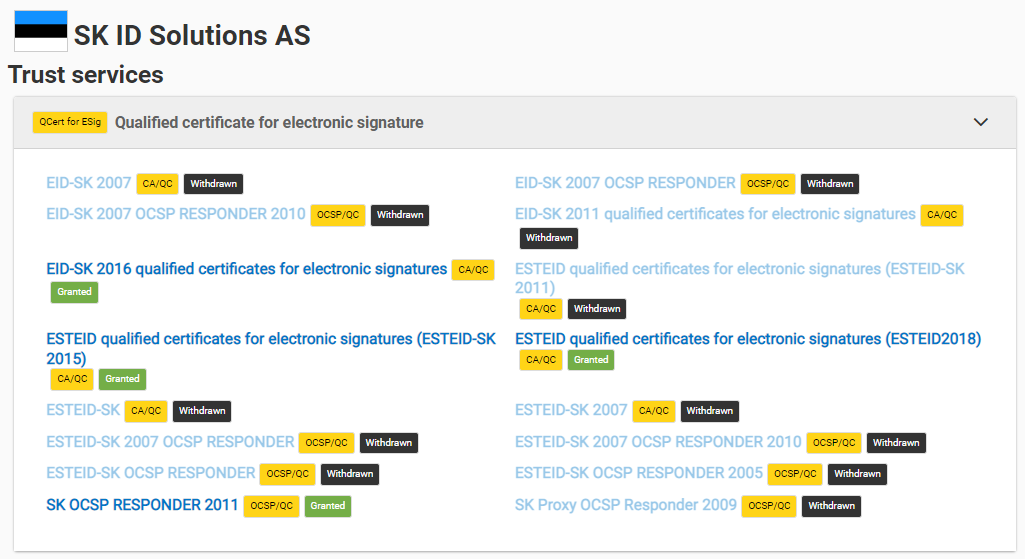
\includegraphics[scale=0.54]{webeid/eu-tsp-skid}
  \caption{List of certificates issued to SK ID Solutions AS for the purposes of Qualified certificate for electronic signature}
  \label{fig:eu-tsp-skid}
\end{figure}

An alternative way to obtain certificates would be to go to the government authority of each country responsible for the distribution of certificates. This action requires prior knowledge of who is responsible for issuing certificates and their purposes.

In Lithuania's case, it is the Ministry of the Interior \cite{eid-lt-ministryofinterior-certificates} who issue two certificates (A and B) every couple of years. As of early 2022, four certificates are active, and all will be added to the trusted CA list.

In Estonia's case, SK ID Solutions manages the CA certificates \cite{eid-ee-skid-certificates}. Of the three certificates found on the EU Trust Services Dashboard, only two are relevant to us, the 2015 and 2018 ones, as the 2016 one has its purpose for use in Smart-ID, which the Web eID framework does not support.

The final list of certificates to support Lithuania and Estonia include four certificates from Lithuania's Ministry of the Interior and two certificates issued by SK ID Solutions for a total of six. It is essential to keep track of these certificates as each one of them can act as a point of compromise and must be monitored in the event they are revoked for security \cite{roca-vulnerability-lessons-learned} or other issues.

\TODO{Discussion: suggest how the certificates are way too challenging to obtain for a casual company and may lead to additional vulnerabilities}
\TODO{Discussion: phishing attacks if the company establishes policy to add certificates if they cannot sign in with their card}

\subparagraph{Exposing the service}

With the certificate validation service configured, it is now required to link it to the Web API. If the company orients around using microservices, this service can be just that. All that the validation service requires is to expose an endpoint that accepts a nonce and a token from the javascript library and returns a validation result.

Companies must take proper measures to protect such service from adversaries as it acts as a fundamental trust anchor. Developers should take steps outlined in assume breach \todo{citation missing} to mitigate the risk of misuse, with the use of TLS and other countermeasures.

\paragraph{Transport protocol}

Researcher Arnis Paršovs published a security analysis of the protocol v1 in October of 2021 \cite{arnis-report-webeid}. Developers behind the Web eID framework acknowledged the weaknesses and addressed them in v2 \cite{ria-webeid-systemarchitecture}, which will be used in the scope of the thesis. At the time of writing, independent researchers and auditors have not yet performed security analysis for this version.

The protocol is two asynchronous JavaScript calls to an API endpoint, which exists on the same website; the user does not need to leave the page. No redirects or third parties are involved; therefore, the analysis of a redirect-based protocol is not applicable in this scenario.

\TODO{Related research about legal person documents?}
\TODO{High-level overview of the system}
\TODO{Points of compromise?}

\TODO{Complete alternative, using your own issued certificates?}